
\subsection{Conduttori massicci}
Si analizza la \textbf{diffusione del campo magnetico} in un conduttore massiccio di conducibilità finita.

Si consideri un dominio regolare $\Omega$ nel quale si individua un volumetto $\Delta\Omega$, l'intera
regione è caratterizzata da un valore finito di $\gamma$ e $\mu$ ed è sede di correnti elettriche e investita
da campi magnetici.

Secondo il modello MQS
$$
\begin{aligned}
&\nabla\times\vec{H} = \vec{J}\\
&\nabla\cdot \vec{B} = 0 \\
&\vec{J} = \gamma\vec{E} \Rightarrow \vec{E} = \frac{\vec{J}}{\gamma}\\
&\nabla\times\vec{E} = -\frac{\partial \vec{B}}{\partial t} \Rightarrow \nabla\times\frac{\vec{J}}{\gamma} = -\frac{\partial \left(\mu\vec{H}\right)}{\partial t} \\
&\vec{B} = \mu\vec{H}
\end{aligned}
$$

Sostituendo la prima nella quarta
$$
\frac{1}{\gamma} \nabla\times\nabla\times\vec{H} = -\mu \frac{\partial}{\partial t} \vec{H} = \frac{1}{\gamma}
\left[\nabla\cancel{\left(\nabla\cdot\vec{H}\right)} - \nabla^2\vec{H}\right]
$$
ma se $\nabla\cdot\vec{B} = 0$ per la legge di Gauss e $\vec{B} = \mu\vec{H}$ allora anche $\nabla\cdot\vec{H} = 0$
e l'equazione di diffusione del campo magnetico diventa
$$
\frac{\partial\vec{H}}{\partial t} = \frac{1}{\mu\gamma} \nabla^2 \vec{H}
$$
in coordinate curvilinee ortogonali $ \vec{H}\left(u_1,u_2,u_3,t\right)$

È possibile risolvere analiticamente il problema quando questo presenta geometrie particolari,
nel caso di problemi bidimensionali ad esempio è possibile utilizzare il metodo della separazione delle
variabili.
\newpage
Si analizza il caso di un cilindro cavo massiccio indefinito, percorso da corrente che giace nel piano $(x,y)$,
per simmetria di rotazione il campo $\vec{H}$ dipenderà solo dalla variabile $r$.
\begin{figure}[H]
\centering
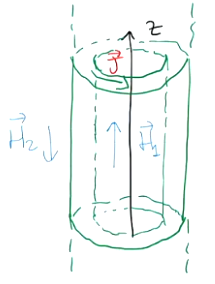
\includegraphics[width = 0.3\linewidth]{cilindro_cavo_massiccio}
\end{figure}
\begin{align*}
&\vec{H} = \vec{H} (r)\\
&\vec{J} = \vec{J}(x,y) = \vec{J}(r)
\end{align*}

Esprimendo la corrente come il rotore del campo $\vec{H}$ e ricordando il prodotto vettoriale tra due
versori si ricava
$$
\vec{J} = \nabla\times\vec{H} = \nabla\times\left(H_z\vec{e}_z\right) = \nabla H_z \times\vec{e}_z = \left(\frac{\partial H_z}{\partial x}\vec{e}_x + \frac{\partial H_y}{\partial y}\vec{e}_y\right) \times \vec{e}_z
$$
$$
\vec{J} = - \frac{\partial H_z}{\partial x}\vec{e}_y + \frac{\partial H_z}{\partial y}\vec{e}_x 
$$
Il campo di corrente giace dunque nel piano che ha per normale l'asse $z$
\newpage
\subparagraph{Diffusione in un semispazio conduttore} con permeabilità magnetica $\mu$.

Il piano $(x,z)$ è attraversato da corrente $\vec{J}(s) = J_s(t)\vec{e}_x$, il campo $\vec{H}$ è dunque ortogonale al piano $(x,y)$
come illustrato in figura.
\begin{figure}[H]
\centering
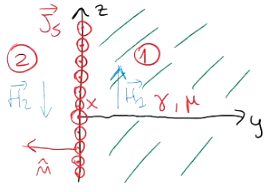
\includegraphics[width=0.4\linewidth]{semipiano_conduttore_campo_magnetico}
\end{figure}

Il caso appena mostrato rappresenta il limite del raggio che tende ad infinito di un solenoide rettilineo,
consci che il campo all'esterno di un solenoide rettilineo infinito sia pari a zero, allora
anche il campo $\vec{H}_2$ sarà pari a zero 

Per la legge di Ampère-Maxwell sulla superficie $y=0$ 
$$
\hat{n}\times\left(\vec{H}_2-\vec{H}_1\right) = \vec{J}_s = -\vec{e}_y \times -\vec{H}_1 = H_{1z}
$$
l'equazione di diffusione diventa
$$
\frac{\partial H_z}{\partial t} = \frac{1}{\mu\gamma} \frac{\partial^2 H_z}{\partial y^2}
$$
è un'equazione la cui incognita è una funzione di due variabili $H_z(y,t)$, è necessario impostare una 
condizione iniziale ed una al contorno
$$
\begin{cases}
H_z(y=0) = J_s(t)\\
H_z(y\to \infty) = 0
\end{cases}
$$
si assume che $J_s(t)$ sia una funzione sinusoidale di pulsazione $\omega$ ossia
$$
J_s(t) = J_{sm} \cos\left(\omega t\right)
$$
l'equazione è lineare e dunque si può utilizzare il metodo dei fasori
$$
\begin{aligned}
&J_s(t) = \Re \left\{\overline{J}_s\ e^{j\omega t} \right\} \\
&H_z(t) = \Re \left\{ \overline{H}_z\ e^{j\omega t} \right\}
\end{aligned}
$$
si trasforma la PDE in ODE sfruttando la derivata fasoriale, ossia la moltiplicazione per $j\omega$
del primo termine
$$
j\omega \overline{H}_z = \frac{1}{\mu\gamma} \frac{d^2}{dy^2}\overline{H}_z
$$
moltiplicando per $\mu\gamma$ e riportando tutto al primo membro
$$
\frac{d^2}{dy^2}\overline{H}_z - j\omega\mu\gamma\overline{H}_z = 0 \Leftrightarrow 
\frac{d^2}{dy^2}\overline{H}_z - k^2 \overline{H}_z = 0
$$
La soluzione generale sarà del tipo
$$
\overline{H}_z(y) = Ae^{ky} + Be^{-ky}
$$
il termine $k$ è la radice di un numero complesso, calcolabile con la \href{https://www.youmath.it/lezioni/analisi-matematica/numeri-complessi/760-calcolare-le-radici-di-un-numero-complesso.html}{formula di de Moivre} e pari
a
$$
k = \sqrt{j\omega\mu\gamma} = \frac{1+j}{\sqrt{2}}\sqrt{\omega\mu\gamma}
$$

La soluzione diventa, introducendo un ulteriore termine $\delta = \sqrt{\frac{2}{\omega\mu\gamma}}$ chiamato 
spessore (o profondità) di penetrazione del campo e dipende dalle caratteristiche del materiale ma anche
dalla pulsazione (o frequenza) del campo.
$$
\overline{H}_z(y) = Ae^{(1+j)\frac{y}{\delta}} + Be^{(1+j)\frac{y}{\delta}}
$$

Si applicano le condizioni al contorno
$$\left\{
\begin{aligned}
&\overline{H}_z(y=0) = A + B = J_{sm}\\
&\overline{H}_z(y\to\infty)=0 \Rightarrow A = 0
\end{aligned}\right.\Rightarrow B = J_{sm} \Rightarrow \overline{H}_z(y) = J_{sm} e^{-(1+j)\frac{y}{\delta}}
$$
In conclusione
$$
H_z(y,t) = \Re \left\{J_{sm}e^{-(1+j)\frac{y}{\delta}}e^{j\omega t} \right\} = J_{sm}e^{-\frac{y}{\delta}}\cos\left(\omega t - \frac{y}{\delta}\right)
$$

Se si considera 
$$
\stackrel{\text{sup}}{t} H_z(y,t) = J_{sm} e^{-\frac{y}{\delta}}
$$
si vede che i picchi delle oscillazioni decrescono con andamento esponenziale all'interno del conduttore.
Si può ragionevolmente ritenere il campo nullo per $y> (4\div5)\delta$.

Il calcolo dello spessore di penetrazione condiziona la progettazione delle macchine elettriche,
il campo magnetico indotto nei metalli genera ulteriori correnti dette ``parassite'' che danno
origine a perdite e dissipazioni per effetto Joule.
\newpage
\paragraph{Lamierino di spessore $\Delta$}
Si nota in figura la distribuzione di correnti che attraversa la superficie esterna del lamierino,
si può analizzare questo caso per sovrapposizione degli effetti.

\begin{figure}[H]
\centering
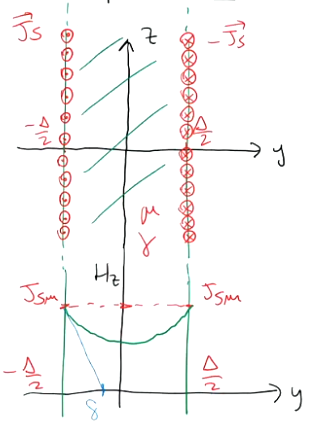
\includegraphics[width = 0.3\linewidth]{lamierino_spessore_delta}
\end{figure}

Esistono due condizioni limite in funzione dello spessore $\delta$
\begin{itemize}
\item $\delta(\omega) \gg \Delta$ condizione di bassa frequenza, il lamierino è interamente penetrato
dal capo magnetico
\item $\delta(\omega) \ll \Delta$ condizione di alta frequenza, il lamierino scherma il campo magnetico
\end{itemize}

Se invece $\delta(\omega) = \Delta$
$$\begin{aligned}
&\sqrt{\frac{2}{\omega\gamma\mu}} = \Delta \Rightarrow \frac{2}{\omega\gamma\mu} = \Delta^2\\
&\omega = \frac{2}{\gamma\mu\Delta^2} = \frac{1}{\tau_m}\quad \tau_m = \frac{\gamma\mu\Delta^2}{2}
\end{aligned}
$$
Il termine $\tau_m$ somiglia al tempo di diffusione del campo magnetico, al quale è associato una frequenza 
caratteristica che discerne il limite di diffusione del campo nel materiale.
\newpage
\subsection{Perdite per correnti parassite}
Per le macchine elettriche, la situazione rilevante è quella di lamierino completamente penetrato,
si suppone in questo caso che 
$$
H_z(t) = \frac{B_m \cos(\omega t)}{\mu}
$$

si applica la legge di Faraday-Neumann all'interno del lamierino ricordando che il campo $\vec{B}$ 
è diretto lungo l'asse $z$ e dunque è necessario calcolare solo la componente $z$ del rotore
$$
\nabla\times\vec{E} = -\frac{\partial\vec{B}}{\partial t} = \cancel{\frac{\partial}{\partial x}E_y} - \frac{\partial}{\partial y}E_x = -\frac{\partial B_z}{\partial t}
$$
Il campo dipende solo dalla coordinata $y$, quindi la derivata rispetto ad $x$ è nulla.
$$
\frac{\partial}{\partial y}E_x = -\omega B_m\sin\left(\omega t\right) \Rightarrow E_x(y,t) = \cancel{C}-\omega B_m\sin\left(\omega t\right)y
$$
Per la simmetria della geometria, $E_x$ deve essere simmetrica rispetto ad $y$ dunque $C=0$

Ricavato il campo si possono determinare le correnti nel materiale e dunque le perdite associate alle correnti 
parassite
$$\begin{aligned}
p^{(a)}(t) &= \iiint_\Omega \vec{E}\cdot\vec{J} dV = \int_0^L dx \iint_S \gamma E_x^2 dS = L\int_{-\frac{\Delta}{2}}^{\frac{\Delta}{2}} dy \gamma \left(\omega B_m \sin\left(\omega t\right)y\right)^2\int_{-\frac{h}{2}}^{\frac{h}{2}}dz=\\
&= hL\gamma\left(\omega B_m\sin\left(\omega t\right)\right)^2\int_{-\frac{\Delta}{2}}^{\frac{\Delta}{2}}y^2 dy=
hL\gamma\omega^2B_m^2\sin^2\left(\omega t\right)\left[\frac{y^3}{3}\right]_{-\frac{\Delta}{2}}^{\frac{\Delta}{2}} =\\
&= hL\gamma\omega^2B_m^2\sin^2\left(\omega t\right) \frac{\Delta^3}{12}
\end{aligned}
$$
ponendo $hL = S$ 
$$
p^{(a)}(t) = \gamma S \omega^2B_m^2\sin^2\left(\omega t\right)\frac{\Delta^3}{12}
$$
La potenza media nel periodo $T = \frac{2\pi}{\omega}$ sarà
$$
<p^{(a)}>_T = \frac{1}{T}\int_0^T p^{(a)}(t')dt'
$$
L'integrale di $\sin^2(\omega t)$ in un periodo è pari ad $\frac{1}{2}$ dunque
$$
<p^{(a)}>_T = \gamma S\omega^2B_m^2\frac{\Delta^3}{24}
$$
ed è pari alla perdita per correnti parassite in un lamierino completamente penetrato.

Preso un lamierino di spessore $\Delta$, viene suddiviso in $n$ lamierini isolati elettricamente di 
spessore $\frac{\Delta}{n}$. Il flusso di $\vec{B}$ è identico (trascurando l'ingombro dell'isolante) dato che il
materiale ferromagnetico occupa lo stesso volume ma le perdite saranno inferiori
$$
<p^{(a)}>_T = n\gamma S\omega^2B_m^2\frac{\left(\frac{\Delta}{n}\right)^3}{24}
$$
confrontandola con la formula ricavata per il lamierino singolo si vede che è $\frac{1}{n^2}$ volte la precedente,
con 10 laminazioni si riduce di 100 volte la potenza persa.

Complessivamente le perdite in corrente alternata si dividono in due termini,
il primo rappresenta le perdite per isteresi dovute alla formula di Steinmetz
$$
<P_{Fe}^{(a)}>_T = K_{ist}B_m^\alpha f 
$$
alle quali si sommano le perdite per correnti parassite appena ricavate
$$
<P_{Fe}^{(a)}>_T = K_{ist}B_m^\alpha f  + K_{cp}B_m^2f^2
$$

Ad esempio per il Fe-Si si hanno i seguenti valori
$$
\mu_r = 200\mu_0,\ \gamma = \SI{2e6}{\siemens\per\meter},\ f = \SI{50}{\hertz}
$$
$$
\delta_{Fe} = \sqrt{\frac{2}{\mu\gamma\omega}} = \SI{3.6}{\milli\meter}
$$
un lamierino spesso \SI{0.36}{\milli\meter} riduce le perdite per correnti parassite di 100 volte.
